\qns{RC Circuit}
\qcontributor{Kyle Tanghe, Elena Jia, Ramsey Mardini}

Consider the circuit below, assume that when $t\leq0$, the capacitor has no charge stored $(V_{\text{c}}(t=0) = 0)$. 
At $t=0$, the switch closes. Assume that $V_s=\SI{5}{\volt}$, $R=\SI{100}{\ohm}$, and $C=\SI{10}{\micro\farad}$. 

\begin{figure}[H]
	\begin{centering}
		\begin{circuitikz}
			\draw (0, 4)
			to[V =$V_s$] (0, 0);
			\draw (0, 4)
			to[switch,l^=\mbox{$t = 0$}](4,4)
			(4,4) to[R = $R$,v=$V_R(t)$,i>^=$i_R(t)$] (7,4)	
			to [short] (9,4)
			to[C = $C$, v=$V_C(t)$,i>^=$i_C(t)$] (9,0)
			to [short] (0,0);
		\end{circuitikz}
		\caption{\label{fig:circuit}RC Circuit with Voltage Source}
	\end{centering}
\end{figure}


\meta{
	This problem is meant to be an introduction to transient analysis of circuits.
	Make sure students fully understand the concepts presented (how to get a differential equation from the circuit, how to solve the equation, and the physical intuition of what is happening in the circuit - charging up a capacitor) before moving on.
}

\begin{enumerate}

\qitem Write out the KCL equations associated with the circuit when the switch is closed.

\meta{
To simplify your circuit analysis, mark the negative end of the voltage source as ground.
}

\sol{
\begin{align*}
\intertext{We denote the voltage to the left of resistor to be $y$. 
We obtain the following differential equations. KCL at node between the resistor and capacitor gives}
\frac{y - V_{\text{C}}}{R} = C\frac{dV_{\text{C}}}{dt} \\
\intertext{Additionally, KCL at the node between the resistor and voltage sources gives:}
\frac{V_{\text{S}} - V_{\text{C}}}{R} +  i_{\text{Vs}} = 0
\end{align*}
}



\qitem Write out the differential equation for $V_{\text{c}}(t)$ after the switch closes.

\meta{
	If students are confused about how to get started, point them to equation (4) in problem 1 as a template.
	Which KCL equation from part (a) of this problem resembles a first order differential equation (i.e. which one has a differential term)?
}

\sol{
\begin{align*}
\intertext{From the previous problem we know that when the switch is closed,}
\frac{V_{\text{S}}- V_{\text{C}}}{R} = C\frac{dV_{\text{C}}}{dt} \\
\intertext{Thus we obtain}
C\frac{dV_{\text{C}}}{dt} + \frac{V_{\text{C}}}{R} - \frac{V_{\text{S}}}{R}=0
\end{align*}
}

\qitem What is the initial condition for $V_{\text{c}}(t)$ (i.e. $V_{\text{c}}(t=0)$) and what is $V_{\text{c}}(t \to \infty)$?

\sol{
No charge is on the capacitor before time $t=0$. Using $q=VC$, we know that $V_{\text{c}}=\SI{0}{\volt}$ before $t=0$.
At $t=0$, the switch closes. Since voltage across the capacitor cannot change instantaneously, $V_{\text{c}}(t=0)=0.$
As $t$ goes to infinity, the capacitor will become fully charged and the current goes to zero. 
Therefore, the voltage of the capacitor equals the voltage source: $V_{\text{c}}(t \to \infty) = V_{\text{S}}.$
}

\qitem Using the initial conditions found in the previous parts, find an expression for 
$V_{\text{c}}(t)$ in terms of $V_{\text{s}}$, $R$, and $C$.

\sol{
	In our case, we know:
	$$ C\frac{dV_{\text{c}}}{dt} + \frac{V_{\text{c}}}{R} - \frac{V_{\text{S}}}{R}=0 $$
	which can be written as
	$$\frac{dV_{\text{c}}}{dt} = - \frac{V_{\text{c}}}{RC} + \frac{V_{\text{S}}}{RC}$$
	From the hint, we know that $\alpha = -\frac{1}{RC}$. We also know that $V_c(0)= 0$ and $V_c = V_s$ from the previous parts.
	Therefore plugging in these values into hint 2, we get:
	$$V_c(t) = V_S + (0 - V_S) e^{-\frac{t}{RC}}$$
	$$V_c(t) = V_S(1 - e^{-\frac{t}{RC}})$$
	$$V_c(t) = V_S(1 - e^{-\frac{t}{\tau}}) \text{ where } \tau = RC \text{ ($\tau$ explained in next part)}$$
}

\end{enumerate}

Aside: $\tau$ is the time constant that we denote for RC circuits. 
Its definition is the time required to charge the capacitor from an initial voltage of zero to about $63.2\%$ of the value of $V_s$, 
or to discharge the capacitor to about $36.8\%$ of its initial charge voltage. For an RC circuit it is equal to $\frac{1}{\alpha}$ 
where $\alpha$ is the eigenvalue of the RC circuit.

\meta{
	Mentors: possibly explain that $36.8\%$ is $e^{-1}$ and $63.2\%$ is $1 - e^{-1}$.
}

\begin{figure}[!h]
  \centering
  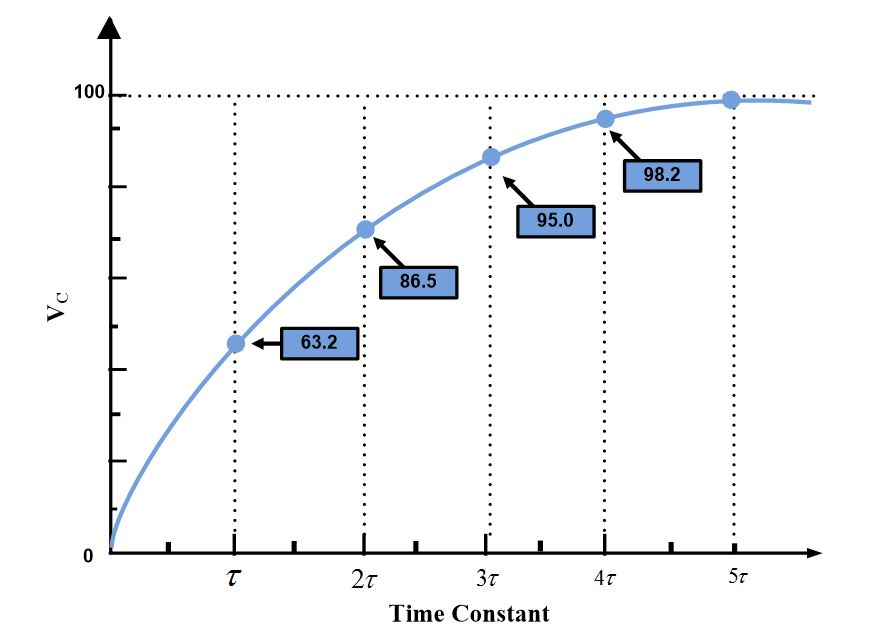
\includegraphics[width=225px]{\bank/ode/figures/tau_curve.jpg}
  \caption{Different values of capacitor voltage at different times, relative to $\tau.$}
  \label{fig:Tau Curve for Charging RC Circuit}
\end{figure}

\begin{enumerate}[resume]
\qitem On what order of magnitude of time (nanoseconds, milliseconds, 10's of seconds, etc.) does this circuit settle 
($V_{\text{c}}$ is $>95\%$ of its value as $t \to \infty$)?

\sol{

The time constant $\tau$ of an RC circuit is just $\tau = RC$. For our circuit:
$$\tau = RC = \SI{100}{\ohm} \cdot \SI{10}{\micro\farad} = \SI{0.001}{\second} $$
After 3 time constants, the voltage will be $~95\%$ of its steady state value
$$3\tau = \SI{0.003}{\second}$$
The circuit will settle on the order of milliseconds.
Alternatively, this value can be found by using algebra:
$$0.95V_S = V_S(1 - e^{-\frac{t}{RC}}) $$
$$-0.05 = -e^{-\frac{t}{RC}} $$
$$0.05 = e^{-\frac{t}{RC}} $$
$$ln(0.05) = -\frac{t}{RC} $$
$$-3 = -\frac{t}{0.001} $$
$$t = 0.003 \, \text{seconds}$$
}

\meta{
	Students may be inclined to blindly use $\tau = RC$ to find a circuit's time constant, regardless of what the RC circuit looks like.
	Remind students that the time constant is only $RC$ for simple RC circuits with only one resistor and one capacitor, but it may be different for different circuits (for instance, in problem 3 on this worksheet).
}

\qitem Give 2 ways to reduce the settling time of the circuit if we are allowed to change one component in the circuit.

\sol{

To reduce settling time, reduce $\tau$. We can achieve this by

\begin{enumerate}
\item Lowering the value of $R$ or
\item Lowering the value of $C$.
\end{enumerate}

Notice how the value of $V_{\text{s}}$ does not change the settling time.

}


\end{enumerate}
